% \documentclass[a4paper, 11pt]{article}

% Added by us
	


%\usepackage{graphicx}
%\usepackage{caption}
%\usepackage{float}
%\usepackage{multicol}
%\usepackage{makecell}
%\usepackage{array}
%\usepackage{color, colortbl}
%\usepackage{arydshln}
%\newcolumntype{P}[1]{>{\centering\arraybackslash}m{#1}}
% \renewrobustcmd{\bfseries}{\fontseries{b}\selectfont}
% \renewrobustcmd{\boldmath}{}
% \newrobustcmd{\B}{\bfseries}

% \newcommand{\dieuwke}[1]{\textcolor{blue}{DH: #1}}
\newcommand{\beginsupplement}{%
        \setcounter{table}{0}
        \renewcommand{\thetable}{S\arabic{table}}%
        \setcounter{figure}{0}
        \renewcommand{\thefigure}{S\arabic{figure}}%
     }

% \newcommand{\specialcell}[2][c]{\begin{tabular}[#1]{@{}l@{}}#2\end{tabular}}


\beginsupplement

\begin{figure}[b]
    \centering
    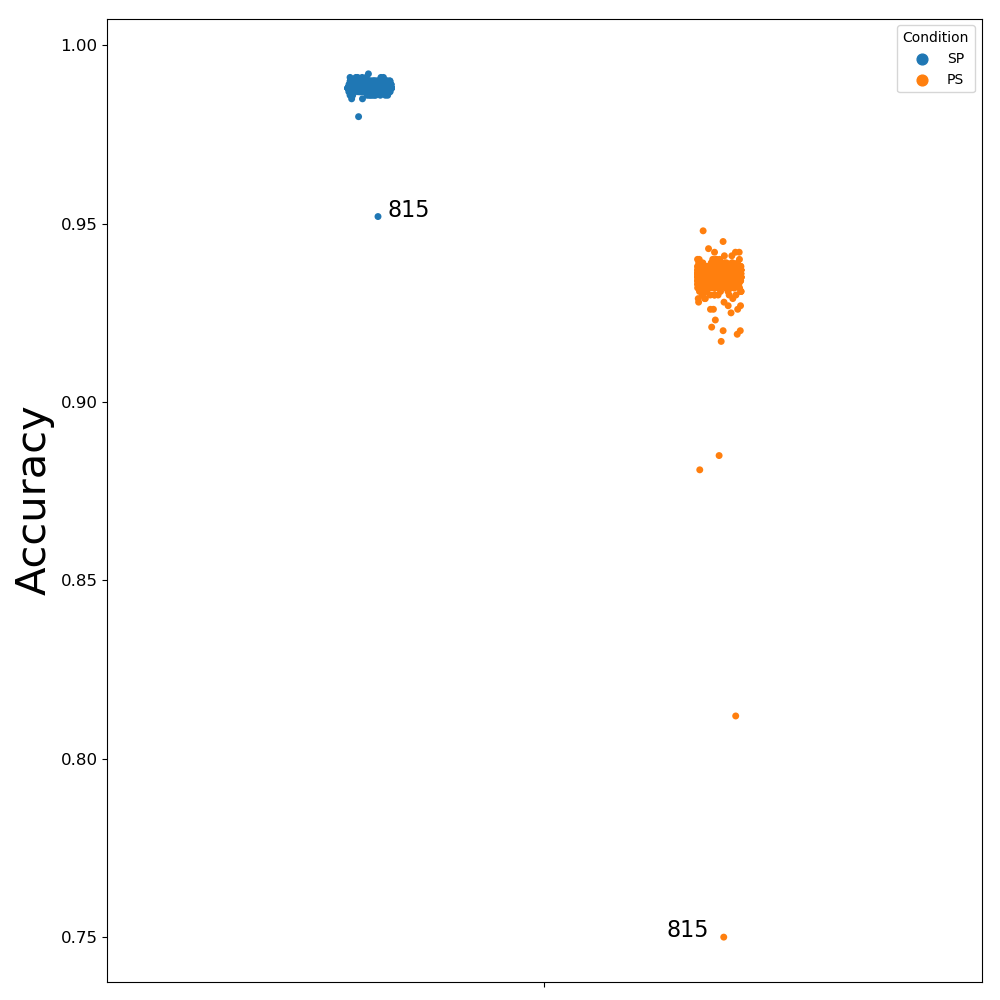
\includegraphics[width=10cm, height=8cm]{figures/SM/Ablation_results_K_model.png}
    \caption{\textbf{Ablation results for the model from Gulordava et. al, 2018}: to identify number units, we ablated each time a different unit in the model and tested the ablated model on the number-agreement task. A blue (orange) dot represents accuracy of an ablated model on the SP (PS) condition of the Noun-PP-number task (Table 2). Compared to all ablations (1300 in total - the number of units in the network), the ablation of only one of the units resulted in a significant reduction in performance (unit 815), in both conditions. This suggest that unit 815 is a number unit, encoding both singular and plural values, consistently with its activity dynamics (Figure 1).}
    \label{fig:ablation_K_model}
\end{figure}

\begin{landscape}
\begin{figure}
    \centering
    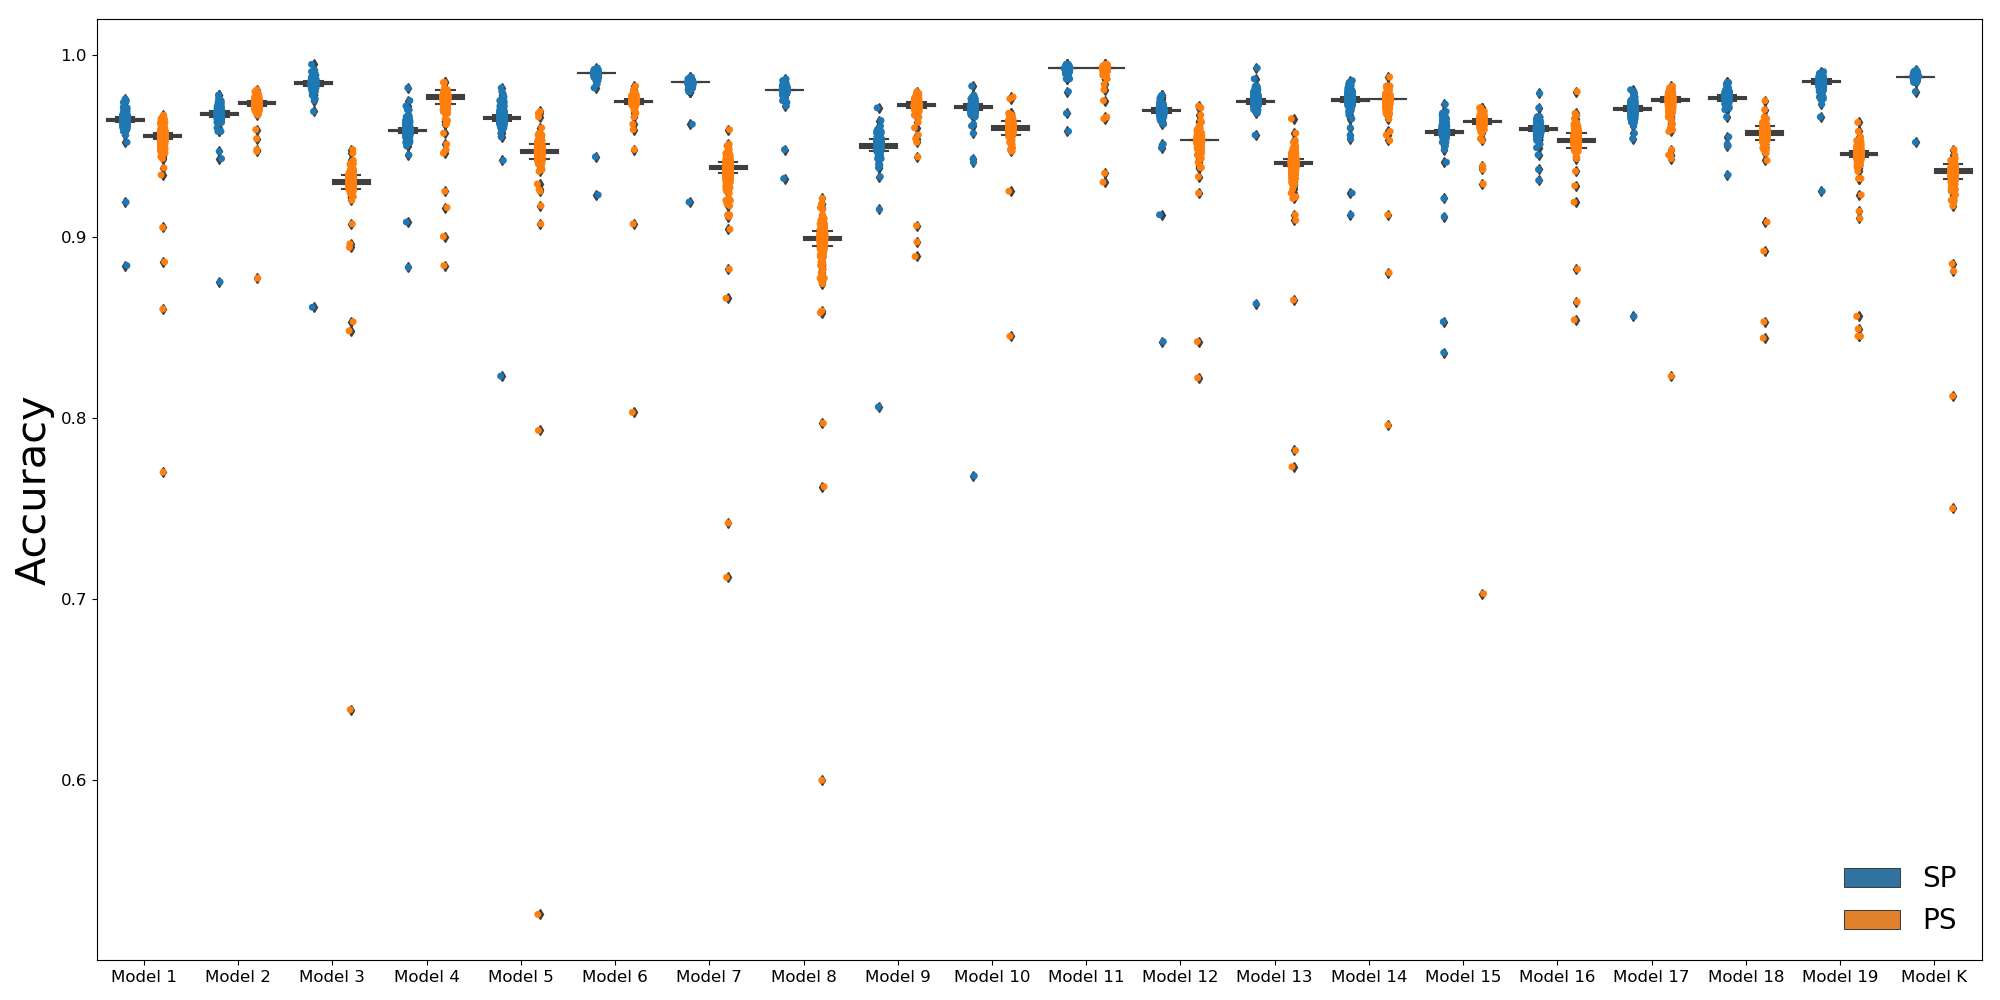
\includegraphics[width=\linewidth]{figures/SM/Ablation_results_all_models.png}
    \caption{\textbf{Ablation results for the control models}: to test the robustness of the sparsity property of the long-range mechanism, we trained 20 additional neural language models (NLMs), using the same hyperparameters as those used for the training of the NLM in Gulordava et. al, 2018. For each NLM, we then repeated the ablation study. Blue and orange dots correspond to accuracy of the ablated models on the SP and PS conditions of the Noun-PP-number task, respectively (see caption of Figure S1). In several NLMs, the ablation of a single unit resulted in a signficant reduction in performance in at least one of the conditions (e.g., models 3, 5, 8 or 15). Overall, in all NLMs, only a small number of ablated models showed significant reduced accuracy compared to all other models (1300 ablated models in total). `Model K' refers to the model from Gulordava et. al, 2018.}
    \label{fig:ablation_all_models}
\end{figure}
\end{landscape}

\begin{figure}
    \centering
    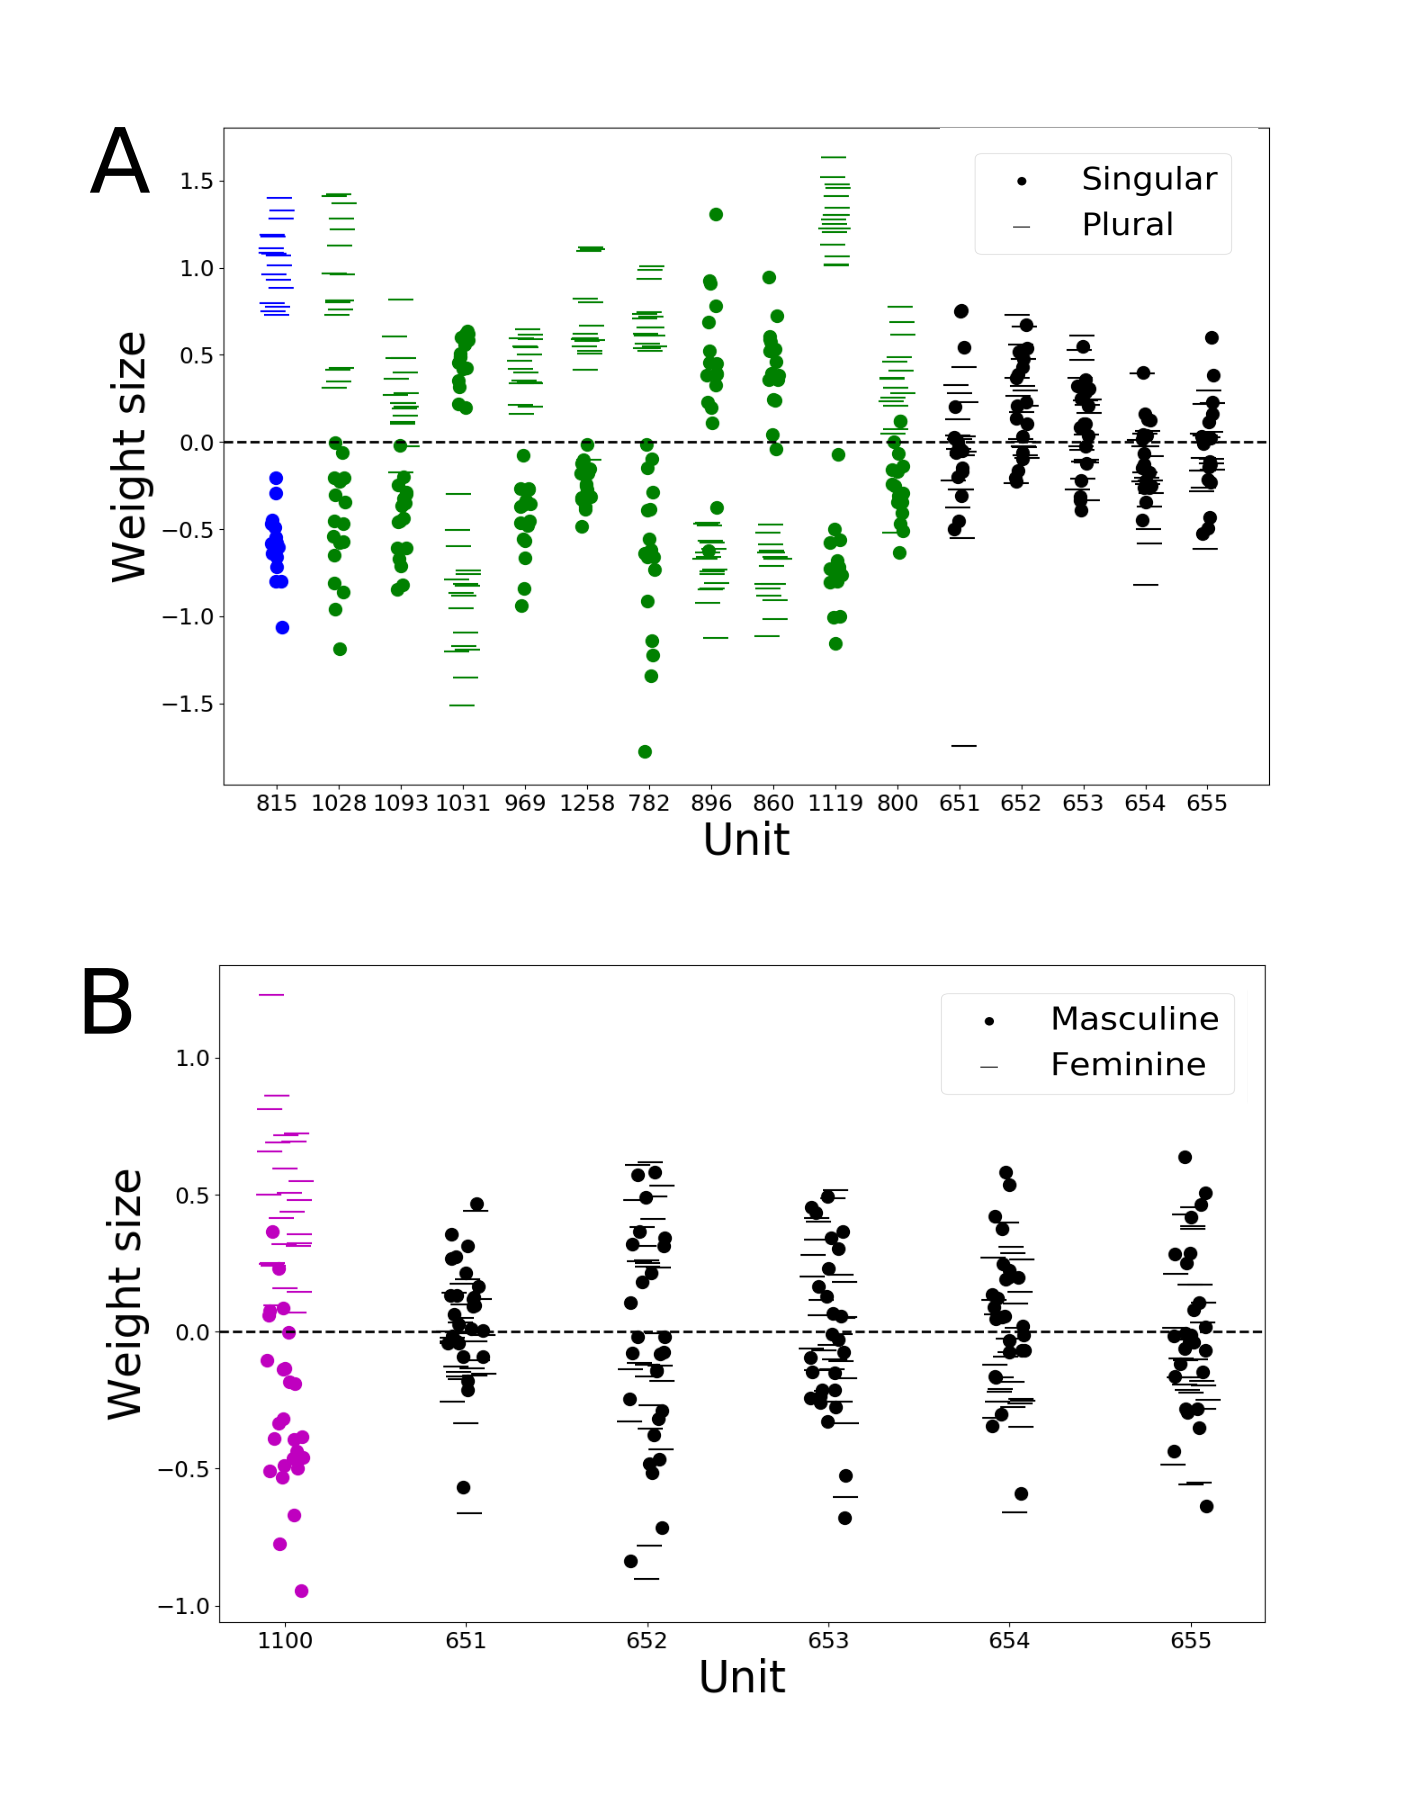
\includegraphics[width=\linewidth]{figures/SM/FigureS2_output_weights.png}
    \caption{\textbf{Efferent weights of number and gender units}: number and gender units were found in the second layer of the network. Units in this layer project onto the output layer, in which each unit corresponds to a word in the lexicon (50,000 in total). We tested whether the efferent weights of the number (gender) units are clustered with respect to grammatical number (gender). A: efferent weights of long-range number units (815; blue), short-range number units (green) and five arbitrary units in the network (black). All weights project to units in the output layer that correspond to singular and plural forms of verbs. Only weights of number units are clustered with respect grammatical number. B: efferent weights of the gender unit (1100; magenta) and five arbitrary units. All weights project onto units in the output layer that correspond to masculine and feminine forms of adjectives. Only the weights of the gender units are clustered with respect to gender value.}
    \label{fig:efferent_weights}
\end{figure}

\begin{landscape}
\begin{figure}
    \centering
    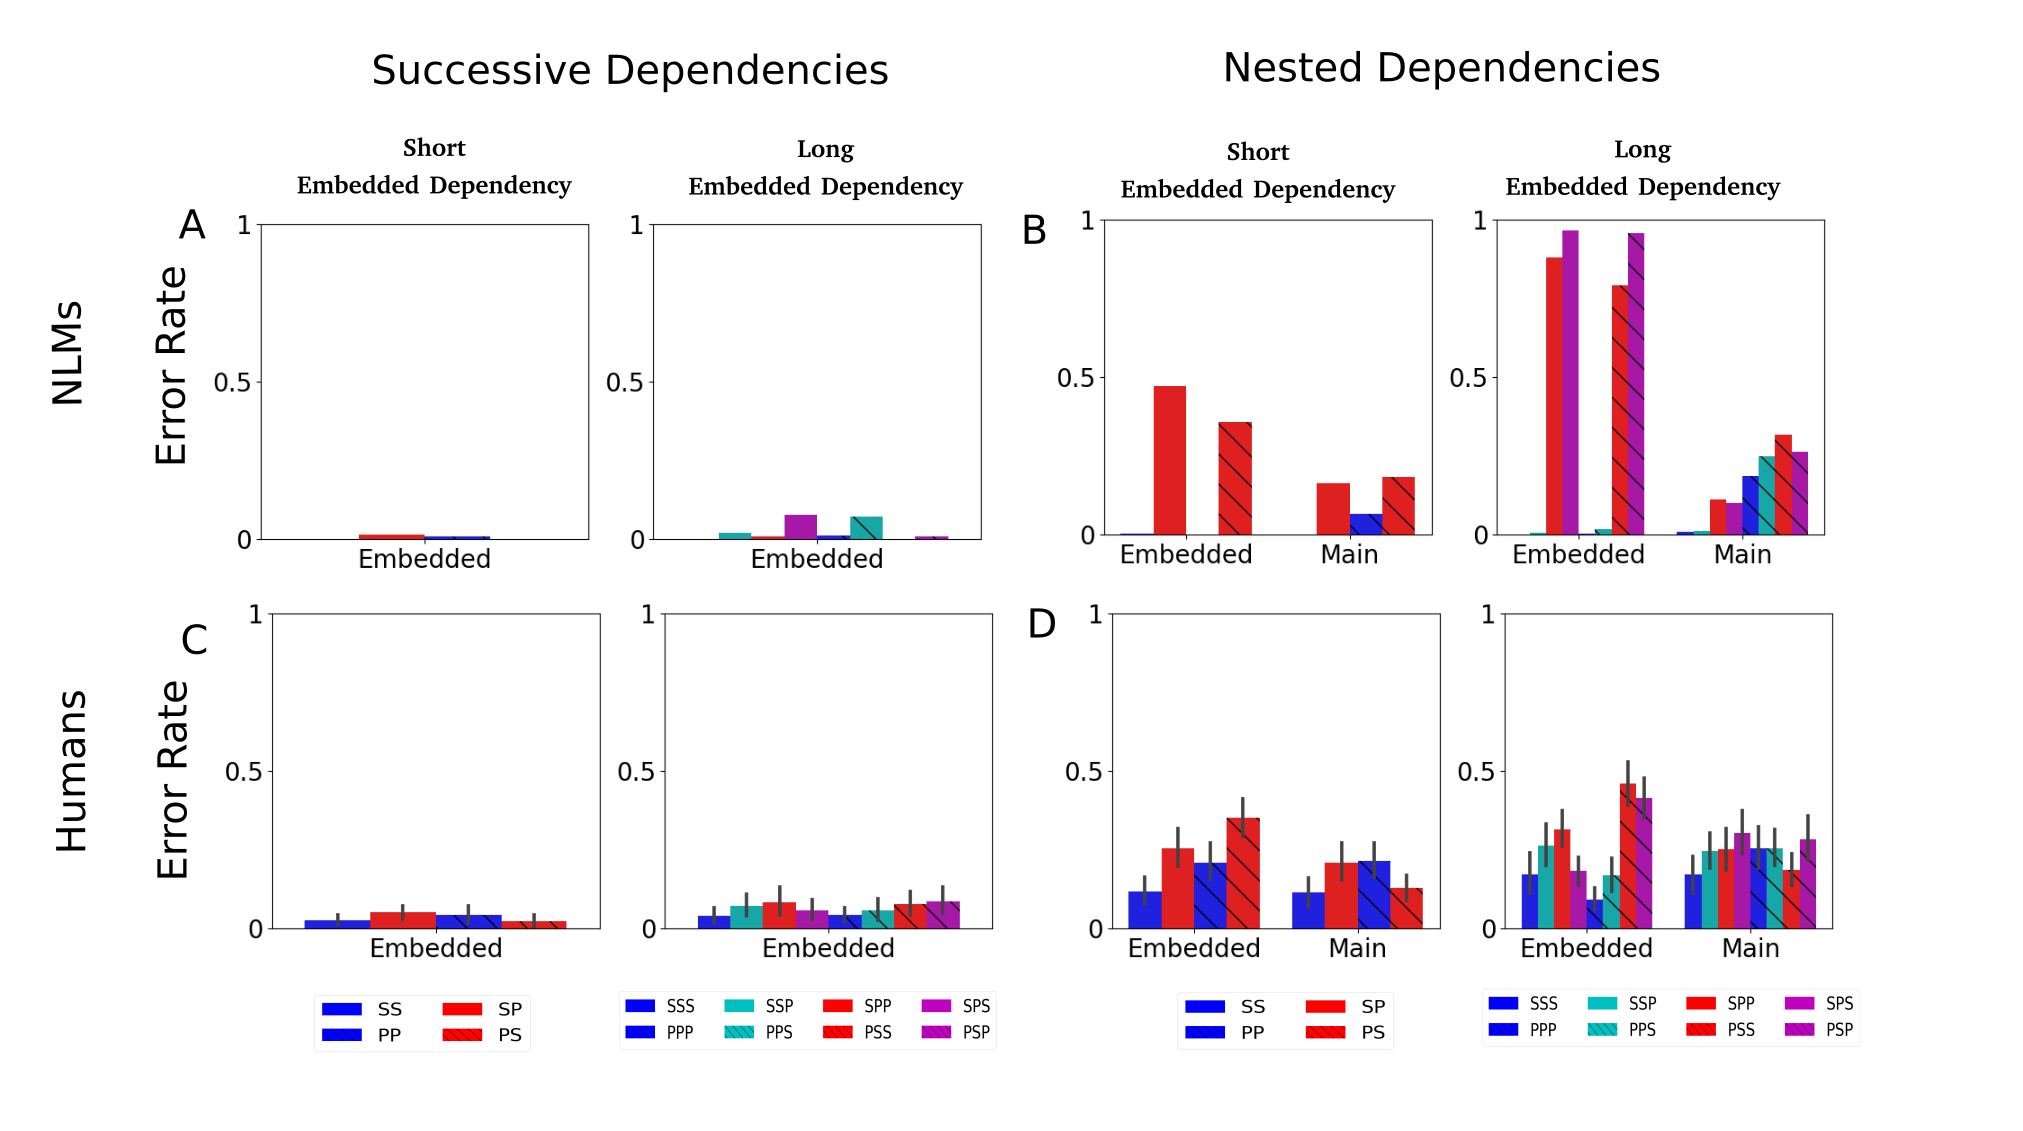
\includegraphics[width=\linewidth]{figures/SM/error_rates_all_conditions.png}
    \caption{\textbf{Error rates for all conditions:} collected from the NLM (panels A \& B) and human subjects (C \& D). Blue \& Cyan (red \& magenta) colors correspond to whether the main and embedded subjects agree (don't agree) on number. Secondary colors (cyan or magenta) represent the presence of a nested attractor carrying an opposite grammatical number to that of the embedded subject. Bars with stripes correspond to conditions in which the main subject is plural. Error bars represent the 95\% confidence level.}
    \label{fig:error_rates_all_conditions}
\end{figure}
\end{landscape}

\begin{figure}[t]
    \centering
    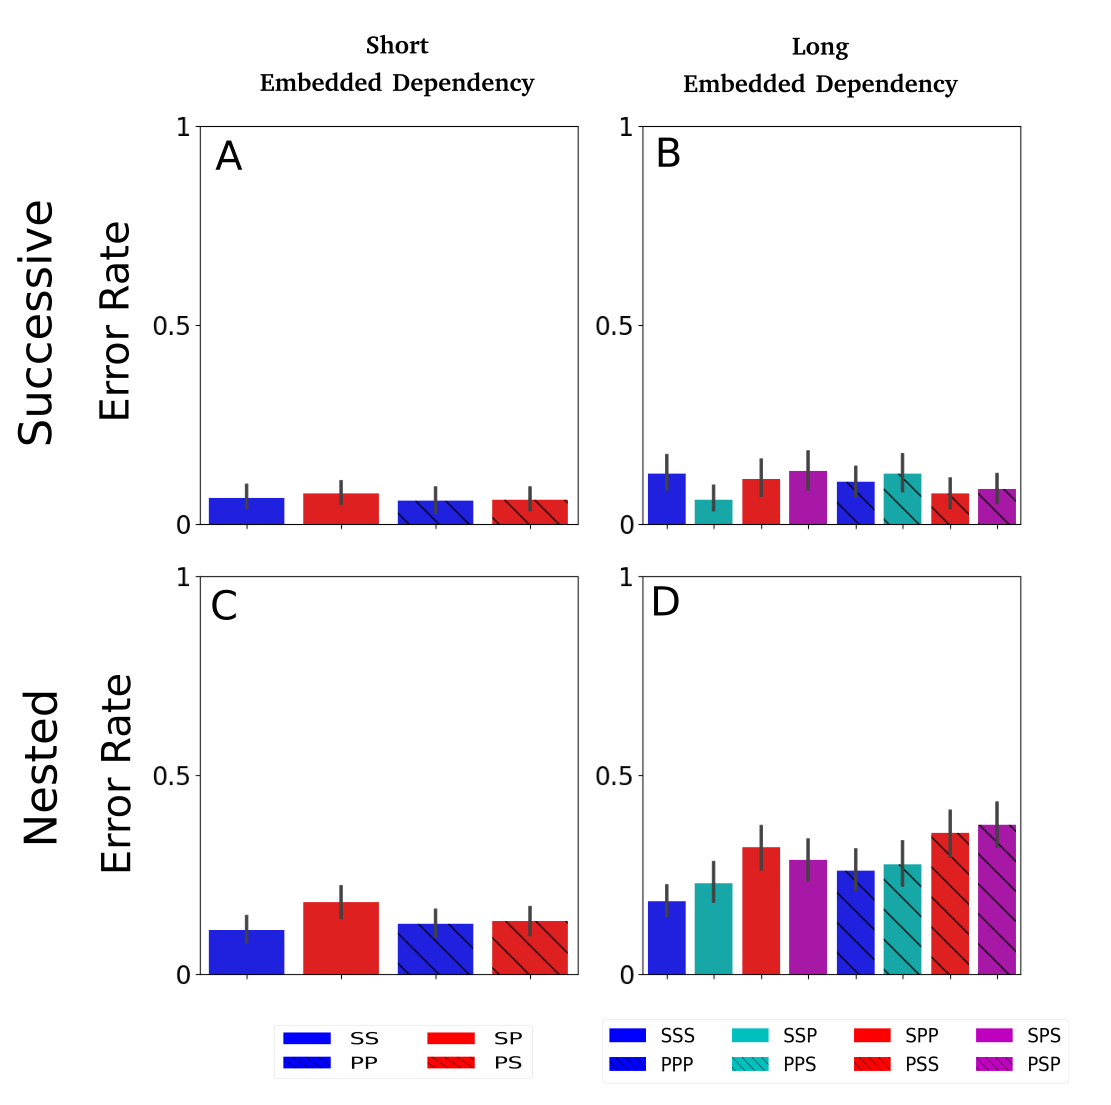
\includegraphics[width=\linewidth]{figures/SM/error_rates_acceptable_all_conditions.png}
    \caption{\textbf{Error rates on grammatical sentences in the behavioral experiment with humans:} for the four constructions - Short-Successive (panel A), Long-Successive (B), Short-Nested (C) and Long-Nested (D). Color coding is the same as in Figure \ref{fig:error_rates_all_conditions}. Error bars represent the 95\% confidence level.}
    \label{fig:error_rates_acceptable}
\end{figure}

% \begin{center}
\begin{table}
\centering
\begin{tabular}{|P{3.3cm}|P{2.5cm}|P{1.2cm}|P{1.5cm}|P{1.5cm}|P{1.3cm}|P{1.5cm}|P{1.5cm}|}
    \hline
    \multicolumn{1}{|c|}{\B Task} & \multicolumn{1}{|c|}{\B Verb} & \multicolumn{3}{|c|}{\B Humans} & \multicolumn{3}{|c|}{\B NLM}\\
    \hline
    \B & \B  & \B $\beta$ & \B z-score & \B p-value & \B $\beta$ & \B z-score & \B p-value\\
    \hline
    \B Successive-Short & \B Embedded & -0.904 & -1.810 & 0.070 & -18.31 & -0.012 & 0.990 \\
    \hline
    \B Successive-Long & \B Embedded  & 0.114 & 0.475 & 0.635 & -2.190 & -4.615 & \B <0.001 \\
    \hline
    \B Nested-Short & \B Main & 0.535 & 2.210 & \B 0.027 & -0.147 & -1.239 & 0.215\\
    \hline
    \B Nested-Short & \B Embedded  & 0.470 & 2.429 & \B 0.015 & -0.481 & -5.252 & \B <0.001 \\
    \hline
    \B Nested-Long & \B Main & 0.244 & 1.684 & 0.092 & -1.2442 & -10.038  & \B <0.001 \\
    \hline
    \B Nested-Long & \B Embedded  & 0.890 & 6.585 & \B <0.001 & -0.542 & -3.579 & \B < 0.001\\
    \hline
\end{tabular}
\caption{\textbf{Effects of grammatical number for humans and the NLM}: for each number-agreement task and each verb, we fitted a logistic regression model with subject-congruence and grammatical number of the attractor subject as variables. In the case of Long-Successive and Long-Nested, the model also included a variable for whether the attractor is congruent or not with the embedded subject. A positive $\beta$ means more errors due to a plural attractor. Significant p-values (<0.05) are marked in bold. }
\label{tbl:stats_number}
\end{table}
\end{center}

\begin{table}[b]
    \centering
    \begin{tabular}{|lll|}
        \hline
    Nouns & masculine & \specialcell{fratello, studente, padre, figlio, ragazzo, bambino,\\ amico, uomo, attore, contadino} \\
    & feminine & \specialcell{sorella, studentessa, madre, figlia, ragazza, bambina,\\ amica, donna, attrice, contadina}\\
    \hline 
    Verbs & & \specialcell{accogliere, amare, attrarre, bloccare, conoscere,\\ criticare, difendere, evitare, fermare, guardare, ignorare,\\ incontrare, indicare, interrompere, osservare, salutare}\\
    % \hdashline
    Matrix verbs & & ricordare, dire, dichiarare \\
    % \hdashline
    Copula & & essere\\
    \hline
    Prepositions & & vicino a, dietro a, davanti a, accanto a\\
    \hline
    Adjectives & & \specialcell{bello, famoso, brutto, ricco, povero, basso, alto, grasso,\\ cattivo, buono, lento, nuovo}\\
    \hline
    \end{tabular}
    \caption{Lexicon used for the agreement tasks.}\label{table:lexicon}
\end{table}


% \end{document}

% \subsubsection{Control model Training} 
% \textbf{M: Given how little emphasis this has in the main text, how about moving it to supplementary? \dieuwke{Agree}} In addition to the NLM made available by \citet{Gulordava:etal:2018}, we train an additional 19 models using the same procedure and corpus (drawn from Wikipedia), giving 20 models in total. 
% The models differ in the order in which those sentences are presented as well as the initialization of their weights.
% For all runs, we use a learning rate of 20, a batch size of 64 and a dropout rate of 0.2, the hyperparameters that \citet{Gulordava:etal:2018} reported to work best for this particular corpus and setup.
% Following Gulordava, but contrary to common practice in language modeling, we train the models on separate sentences, rather than longer pieces of discourse.
% As common practice for training language models, we do not use an optimizer, but instead use a \emph{plateau-based} learning scheme, in which we half the learning rate whenever the validation perplexity of the model reaches a plateau.

% After training, we evaluate the resulting 20 models by considering their perplexity on a shared test set\footnote{\url{https://dl.fbaipublicfiles.com/colorless-green-rnns/training-data/Italian/test.txt}}. 

% \subsection{Markedness effect in humans and NLM}
% \textbf{M: What is the reason to put this in the main? The issue of whether plural is also a marked feature for NLMs is interesting (for example, to test theories that markedness is a function of statistical trends that should also be picked up by language models). However, in the context of our discussion, I find it quite distracting. I would vote for moving it entirely to the appendix (together with the full-results analyses above).}

% Finally, we tested for markedness effects in both humans and the NLM.
% For each verb in each of the four NA-task, we fitted a logistic-regression model with subject-congruence and grammatical number of the intervening subject as variables. Note that, while for embedded verbs the intervening subject is the main subject, for main verbs, the intervening subject is the embedded subject. In the case of Long-Successive and Long-Nested, we also included congruence of the embedded subject and the nested attractor as a variable in the regression model. 

% In humans, we found significant main effects for the grammatical number of the intervening subject in the following cases: embedded and main verbs in Short- and Long-Nested (Short-Nested: $\beta^{embedded}=0.47; p-value<0.05$ and $\beta^{main}=0.56; p-value<0.05$; Long-Nested: $\beta^{embedded}=0.67; p-value<0.001$ and $\beta^{main}=0.47; p-value<0.05$; positive $\beta$ indicates more errors due to intervention of a plural number). In Long-Nested, we further found an interaction between subject-congruence and the grammatical number of the intervening attractor ($\beta^{interaction}=1.4173; p-value<0.001$). In contrast, in the NLM, an intervening plural noun did not generate more errors compared to singular. In several cases, the effect was reversed, i.e., an intervening singular noun caused more errors - Table S1\ref{} summarizes all effects found in both humans and the NLM. 
